\chapter{Methods}
\label{ch:methods}

\section{Strains and media}
\label{sec:methods-strains_media}

The \textit{S. cerevisiae} strains used in this thesis are described in table~\ref{tab:methods-strains}.
% Potential additions: CEN.PK & Causton strains, if they go into the biological chapter.

\begin{table}
  \footnotesize
  \centering
  \begin{tabularx}{\linewidth}{bbbbb}
    \toprule
    Name & Background & Genotype & Origin & Notes\\
    \midrule
    FY4 & FY4 & - & EUROSCARF & \textcite{winstonConstructionSetConvenient1995} \\
    htb2::mCherry & FY4 & HTB2::mCherry & In-house, CRISPR & - \\
    BY4741 & BY4741 & \textit{MAT}a \textit{his3$\Delta$1 leu2$\Delta$0 met15$\Delta$0 ura3$\Delta$0} & EUROSCARF & \textcite{brachmannDesignerDeletionStrains1998}\\
    \textit{zwf1$\Delta$} & BY4741 & \textit{zwf1$\Delta$::KAN} & Edinburgh Genome Foundry & Yeast deletion collection \\
    BY4742 & BY4742 & \textit{MAT}a \textit{his3$\Delta$1 leu2$\Delta$0 lys2$\Delta$0 ura3$\Delta$0} & Bruce Morgan & \textcite{calabreseHyperoxidationMitochondrialPeroxiredoxin2019}\\
    \textit{tsa1$\Delta$ tsa2$\Delta$} & BY4742 & \textit{tsa1$\Delta$::natNT2 tsa2$\Delta$::kanMX4} & Bruce Morgan & \textcite{calabreseHyperoxidationMitochondrialPeroxiredoxin2019} \\
    CEN.PK113-7D & CEN.PK113-7D & - & Peter K\"{o}tter & \textcite{nijkampNovoSequencingAssembly2012} \\
    \bottomrule \\
  \end{tabularx}
  \caption{Strains used in this thesis.}
  \label{tab:methods-strains}
\end{table}

The minimal medium described by \parencite{verduynEffectBenzoicAcid1992} was used unless otherwise stated.
This minimal medium does not contain riboflavin, thus minimising its effect on flavin autofluorescence imaging, and its composition is known and easily controlled.
Specifically, the composition of the carbon source-limiting medium are described in tables~\ref{tab:methods-media-delft}--\ref{tab:methods-media-delft-vitamins}, and the media pH was adjusted to 6.0 before use using potassium hydroxide, or sodium hydroxide for potassium-free media.
For auxotrophic strains, supplements were added according to table~\ref{tab:methods-media-auxotroph}.
Then, a carbon source is added as appropriate to create the growth medium.

\begin{table}
  \footnotesize
  \centering
  \begin{tabularx}{\linewidth}{bbb}
    \toprule
    Reagent & Concentration & Remarks\\
    \midrule
    \ce{KH2PO4} & \SI{3.}{\gram~\litre^{-1}} & \\
    \ce{MgSO4.7H2O} & \SI{0.5}{\gram~\litre^{-1}} & \\
    \ce{(NH4)2SO4} & \SI{5.}{\gram~\litre^{-1}} & \\
    \ce{Trace metals} & \SI{1.}{\milli\litre~\litre^{-1}} & See table~\ref{tab:methods-media-delft-metals} \\
    \ce{Vitamins} & \SI{1.}{\milli\litre~\litre^{-1}} & See table~\ref{tab:methods-media-delft-vitamins}.  Add upon use. \\
    \ce{Carbon source} & variable & Add upon use. \\
    \bottomrule \\
  \end{tabularx}
  \caption[
    Composition of base minimal medium
  ]{
    Composition of base minimal medium.
    For potassium-free media, replace \ce{KH2PO4} with \SI{2.65}{\gram~\litre^{-1}} \ce{NaH2PO4}, which gives the same molarity.
  }
  \label{tab:methods-media-delft}
\end{table}

\begin{table}
  \footnotesize
  \centering
  \begin{tabularx}{\linewidth}{bbS}
    \toprule
    Reagent & Formula & {Concentration [\SI{}{\gram~\litre^{-1}}]}\\
    \midrule
    EDTA & \ce{C10H14N2Na2O8.2H2O} & 15.00 \\
    Zinc sulfate & \ce{ZnSO4.7H2O} & 4.50 \\
    Manganese (II) chloride & \ce{MnCl2.2H2O} & 0.84 \\
    Cobalt (II) chloride & \ce{CoCl2.6H2O} & 0.30 \\
    Copper (II) sulfate & \ce{CuSO4.5H2O} & 0.30 \\
    Sodium molybdate & \ce{Na2MoO4.2H2O} & 0.40 \\
    Calcium chloride & \ce{CaCl2.2H2O} & 4.50 \\
    Iron (II) sulfate & \ce{FeSO4.7H2O} & 3.00 \\
    Boric acid & \ce{H3BO3} & 1.00 \\
    Potassium iodide & \ce{KI} & 0.10 \\
    \bottomrule \\
  \end{tabularx}
  \caption[
    Composition of trace metal mix
  ]{
    Composition of trace metal mix for minimal media described in table~\ref{tab:methods-media-delft}.
  }
  \label{tab:methods-media-delft-metals}
\end{table}

\begin{table}
  \footnotesize
  \centering
  \begin{tabularx}{\linewidth}{bbS}
    \toprule
    Reagent & Formula & {Concentration [\SI{}{\gram~\litre^{-1}}]}\\
    \midrule
    D-(+)-biotin & \ce{C10H16N2O3S} & 0.05 \\
    D-panthothenic acid calcium salt & \ce{Ca(C9H16NO5)2} & 1.00 \\
    Nicotinic acid & \ce{C6H5NO2} & 1.00 \\
    \textit{myo}-Inositol & \ce{C6H12O6} & 25.00 \\
    Thiamine chloride hydrochloride & \ce{C12H15ClN4OS.HCl} & 1.00 \\
    Pyridoxal hydrochloride & \ce{C8H12ClNO3} & 1.00 \\
    4-aminobenzoic acid & \ce{C7H7NO2} & 0.20 \\
    \bottomrule \\
  \end{tabularx}
  \caption[
    Composition of vitamin mix
  ]{
    Composition of vitamin mix for minimal media described in table~\ref{tab:methods-media-delft}.
  }
  \label{tab:methods-media-delft-vitamins}
\end{table}

\begin{table}
  \footnotesize
  \centering
  \begin{tabularx}{\linewidth}{bS}
    \toprule
    Reagent & {Concentration [\SI{}{\milli\gram~\litre^{-1}}]} \\
    \midrule
    histidine & 125. \\
    leucine & 500. \\
    tryptophan & 75. \\
    methionine & 100. \\
    uracil & 150. \\
    \bottomrule \\
  \end{tabularx}
  \caption[
    Supplements to minimal media for auxotrophic strains
  ]{
    Supplements to minimal media for BY4741-background auxotrophic strains, compositions derived from \textcite{pronkAuxotrophicYeastStrains2002}.
    For BY4742-background strains, replace methionine with \SI{100}{\milli\gram~\litre^{-1}} lysine-HCl.
  }
  \label{tab:methods-media-auxotroph}
\end{table}

\section{Single-cell microfluidics}
\label{sec:methods-microfluidics}

Cells were grown from colonies on solid agar in a liquid culture composed of minimal media formulation appropriate for the experiment, supplements appropriate for the strain's auxotrophy, and a carbon source (glucose or pyruvate) appropriate for the experiment (see section~\ref{sec:methods-strains_media}).
% Kevin's OD measurements?
The cells were incubated at \SI{30}{\celsius} for \SI{14}{\hour} (overnight) if the carbon source is glucose or \SI{48}{\hour} if the carbon source is pyruvate.
Subsequently, the cells were diluted so that the resulting culture had an OD\textsubscript{600} of 0.10--0.20, and were then incubated for a further \SI{4}{\hour}.

\begin{figure}
  \centering
  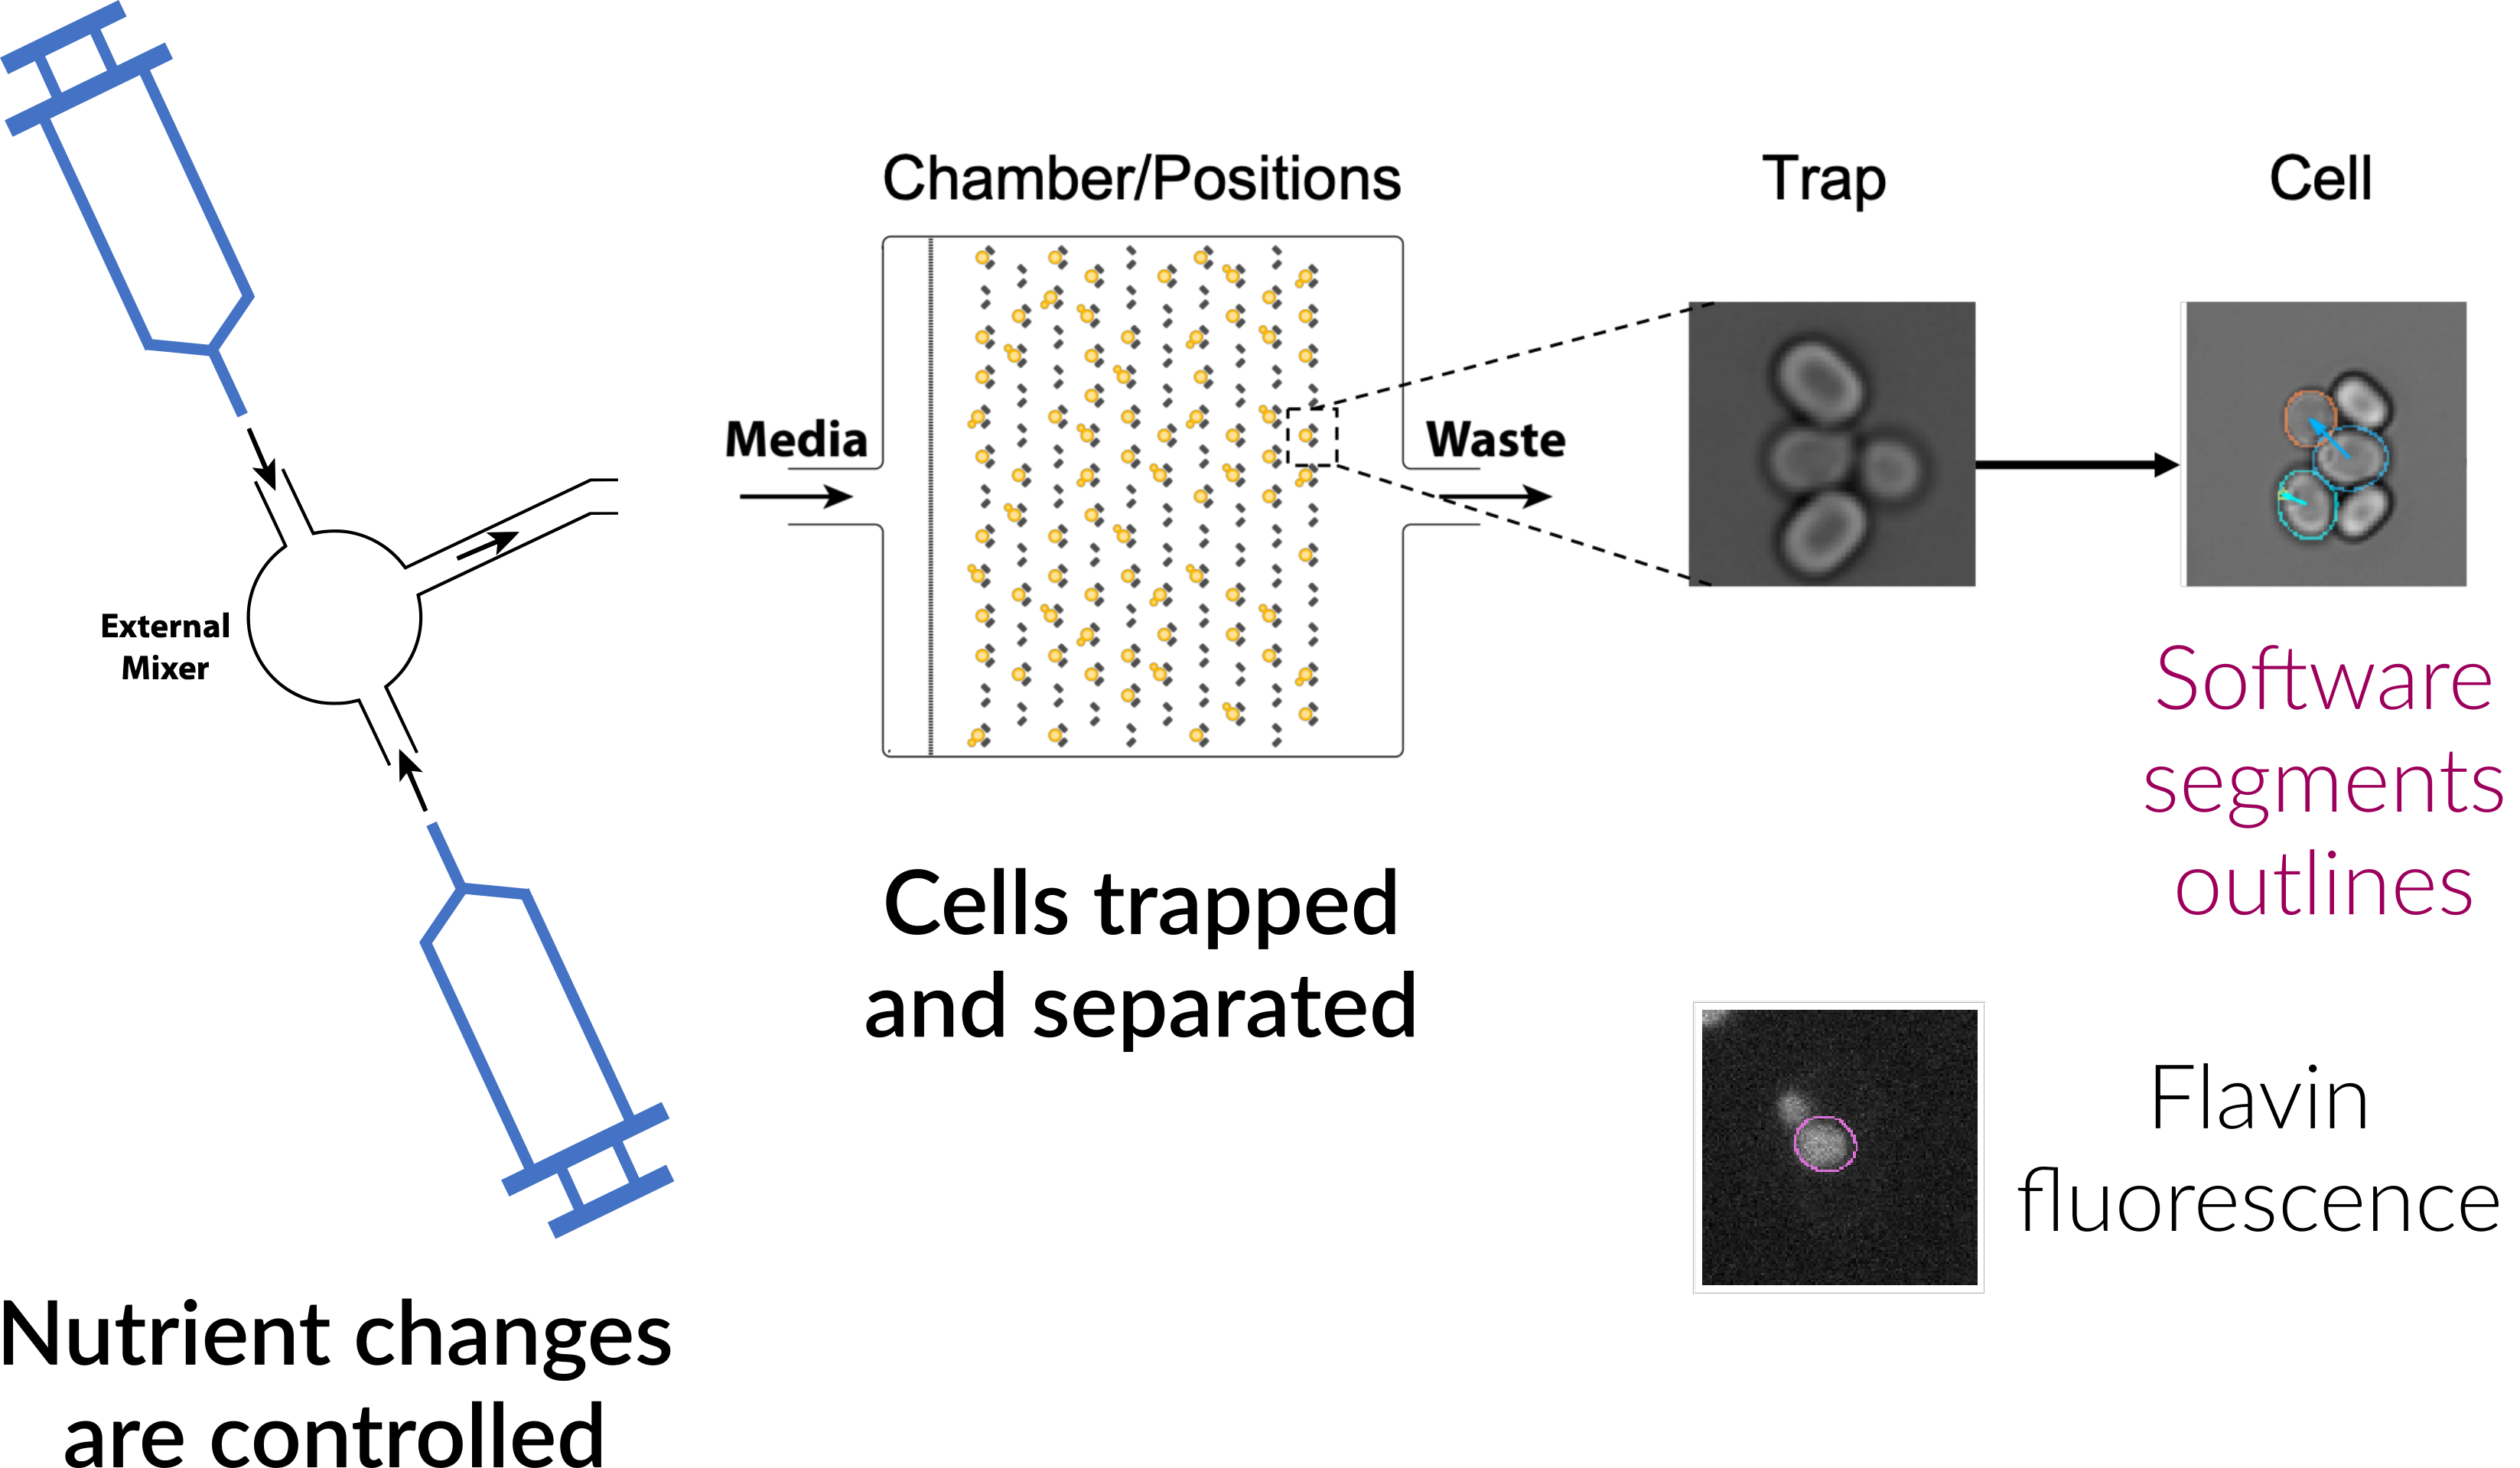
\includegraphics[width=0.9\textwidth]{microfluidics}
  \caption[
    Overview of single-cell microfluidics set-up using the ALCATRAS system
  ]{
    Overview of single-cell microfluidics set-up using the ALCATRAS system.
    Cells are loaded into chambers within devices, where they are trapped and separated (centre).
    The media composition the cells experience are controlled with syringe pumps (left).
    Brightfield and fluorescent images are taken at regular intervals, and then processed using \textit{aliby} \parencite{munozgonzalezPhenotypingSingleCells2023} to provide time series of fluorescence intensity changes for each parent cell.
  }
  \label{fig:methods-microfluidics}
\end{figure}

ALCATRAS microfluidics \parencite{craneMicrofluidicSystemStudying2014} devices were then prepared and for an experiment, one device's multiple chambers were filled with growth media supplemented with 0.05\% w/v bovine serum albumin.
Cells were then loaded into the ALCATRAS chambers --- different chambers can house cells from different strains (figure~\ref{fig:methods-microfluidics}).
Syringe pumps containing media were programmed to produce a constant flow of \SI{4}{\micro\litre~\hour^{-1}} into the chambers.
As a consequence, parent cells are held in place within traps, while progeny cells flow out of traps into the outflow after the parents bud.
There are two syringes that can contain different media, and in experiments that require different nutrient conditions at different times, the ALCATRAS system is programmed to switch between the two syringes.
The cells and ALCATRAS chambers were located in an incubation chamber (Oko-labs) that was maintained at \SI{30}{\celsius}.

% Update fluorescence settings
Microscopy was performed using a 60 $\times$ 1.4 NA oil immersion objective (Nikon), and the Nikon Perfect Focus System was used to ensure consistent focus.
X-Y spatial positions were defined for each chamber to maximise spatial coverage of the chamber while ensuring that the microscope takes less time to move positions and capture images than the interval period.
Images were taken every \SI{5}{\minute}, and image acquisition duration varied for each experiment.
Brightfield and flavin images were captured in all strains and mCherry images were additionally captured for the HTB2::mCherry strain.
Five z-slices were taken for brightfield images, with a spacing of \SI{0.6}{\micro\metre} between slices.
Fluorescence imaging was performed with an OptoLED light source (Cain Research), and LED voltage was optimised for maximum signal intensity without LED cut-off prior to experiments.
For flavin imaging, the excitation filter was set to 430/24 (\SIrange{418}{442}{\nano\metre}), the emission filter was set to 535/30 (\SIrange{520}{550}{\nano\metre}), and the exposure time was \SI{60}{\milli\second}.
One z-slice was taken for each flavin image in each position.
For mCherry imaging, the excitation filter was set to \SIrange{555}{590}{\nano\metre}), the emission filter was to set to 632/60 (\SIrange{602}{682}{\nano\metre}) and the exposure time was \SI{100}{\milli\second}.
Five z-slices were taken for mCherry images, with a spacing of \SI{0.6}{\micro\metre} between slices.

\section{Segmentation, extraction, post-processing}
\label{sec:methods-segmentation}

I used \textit{aliby} \parencite{munozgonzalezPhenotypingSingleCells2023}, an end-to-end Python-based software package developed for time-lapse microscopy, to process the microscope images in order to obtain flavin and mCherry time series for further analysis.

\textit{aliby} tracks tiles that correspond to a trap across time-lapse images to account for expected spatial drifting in the microscope.
It then uses \textit{BABY} \parencite{pietschDeterminingGrowthRates2023} to segment the images of traps to identify the outlines of cells and to track cells from one time point to another, creating a lineage of cells.
\textit{aliby} then overlays the cell outlines onto the fluorescence (flavin and mCherry) images to extract fluorescence intensity, and assigns a fluorescence value to each cell at each time point based on the mean intensity of pixels within the cell's outline.
The background fluorescence is also computed, based on the pixel intensity outside cell outlines, and is then subtracted from the cell fluorescence.
Flavin fluorescence thus represents the oxidation of flavins throughout the yeast metabolic cycle (see section~\ref{sec:intro-flavin}), and mCherry fluorescence thus represents the amount of histone proteins as a proxy for cell division cycle progression \parencite{garmendia-torresMultipleInputsEnsure2018}.

%%% Local Variables:
%%% mode: latex
%%% TeX-master: "../thesis.tex"
%%% End:
